\section{Stemningsregistrering}\label{stemningsleje::stemningsregistrering}
Under mødet med Psykolog Janne Rasmussen\cite[Afsnit 1.3, Møde med Psykolog Janne Rasmussen]{faelles} blev der nævnt en metode kaldet stemningsregistrering.
Dette afsnit vil kortfattet beskrive denne metode og dens effekt.

Stemningsregistrering\cite[Appendiks F, Stemningsregistrering]{faelles} hjælper patienten med at reflektere over sin stemningsleje.
Det gør at patienten er mere klar over hvordan han har det.
Stemningsregistrering fungerer som hjælpeværktøj under behandlingen, da det er lettere for behandleren at se hvordan patienten har det vha. stemningsregistreringen og samtidig får patienten selv en bedre forståelse.
Stemningsregistrering fungerer ved at patienten hver dag krydser af i et skema, i det felt der svarer til patientens egen opfattelse af sin stemningsleje.
Dette gør at man kan finde mønstre, fx. at patienten er deprimeret hver søndag.
Dette kan så bruges under samtale med behandleren.
Det eneste krav er at patienten kender sine egne symptomer.

Et eksempel på et skema kan ses på \cref{figure::stemningsregistrerings_skema}.
På skemaet kan patienten udfylde fem punkter:
\begin{itemize}
	\item Stemningsleje
	\item Angst
	\item Antal timers søvn
	\item Medicin
	\item Notater og vægt
\end{itemize}

\begin{figure}
	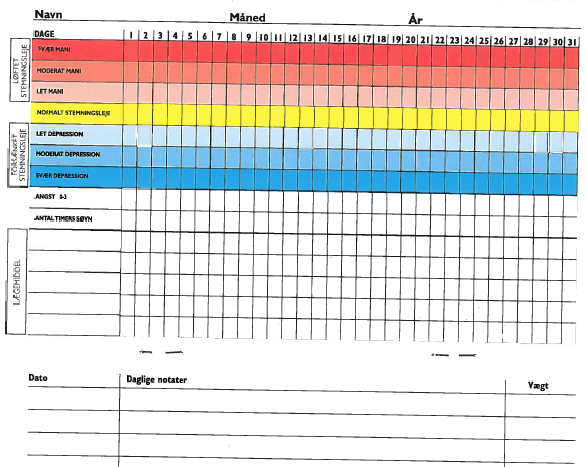
\includegraphics[width=\textwidth]{stemningsregistrerings_skema.png}
	\caption{Et eksempel på et tomt stemningsregistrerings skema.}
	\label{figure::stemningsregistrerings_skema}
\end{figure}

\subsection{De fem punkter}
I dette afsnit bliver de fem punkter udspecificeret.
De er baseret på \citet[Appendiks F, Stemningsregistrering]{faelles}.
\paragraph{Stemningsleje}
Under dette punkt er der syv valg:
\begin{itemize}
	\item \textbf{Normal}(gul), hvis der ikke er symptomer på mani eller depression. Energiniveauet er normalt. Søvnen er normal. Forholdsvis nemt at passe daglige aktiviteter.
	\item \textbf{Let mani}(lyserød), hvis patienten føler sig opstemt og optimistisk eller mere irritabel end sædvanligt. Patienten oplever følgende; mere energi, flere ideer, øget selvtillid, mere udadvendt, mere talende, øget sexuallyst, rastløs, sover mindre, vanskeligt ved at arbejde effektivt og fungere socialt.
	\item \textbf{Moderat mani}(mellemrød), griner på upassende tidspunkter eller er meget irritabel og utålmodig, taler meget også selvom andre prøver at sige noget, sover kun fire timer om natten, svært ved at samle sig om en ting, ikke i stand til at passe arbejdet, tænker meget på sex.
	\item \textbf{Svær mani}(rød), ekstatisk, meget grinende eller er vredladen og ofte udskældende, verbale eller fysiske kampe med andre, tror på vedkommende har særlige evner (læse tanker, høre stemmer), konstant bevægelse, sover meget lidt eller ikke, mister kontrollen.
	\item \textbf{Let depression}(lyseblå), lettere trist, selvkritisk, negative tanker, lidt større søvnbehov, svært ved at falde i søvn, træt, er livet værd at leve?, mindre effektiv, kan godt arbejde, andre bemærker det ikke.
	\item \textbf{Moderat depression}(mellemblå), nedtrykt, opgivende, uinteresseret, følger sig langsom, sover mere, svært ved at falde i søvn, bebrejdelse, ukoncentreret, får ikke tingene gjort, selvmordstanker, svært at passe arbejde.
	\item \textbf{Svær depression}(blå), meget nedtrykt, føler intet, håbløshed, energiløs, mistet interessen for alt, ingen appetit, kan ikke sove, alvorlige selvmordstanker, hører stemmer eller ser syner, kan ikke arbejde, svært ved egenomsorg, i sengen det meste af dagen.
\end{itemize}

\paragraph{Angst}
Angst angives på en skala fra og med nul til og med tre.
\begin{itemize}
	\item \textbf{0} svarer til at man ikke oplever nogen form for angst.
	\item \textbf{1} Lettere ængstelig, men påvirker ikke dagligdagen.
	\item \textbf{2} Konstant ængstelig, funktionsniveau påvirkes.
	\item \textbf{3} Udtalt angst, kan næsten ikke foretage sig noget.
\end{itemize}

\paragraph{Antal timers søvn}
Antal timers søvn selvom søvnen har været afbrudt.

\paragraph{Medicin}
Her skrives hvilket og hvor meget medicin der tages i begyndelsen af hver måned.

\paragraph{Notater og vægt} 
Vægten skal registreres mindst en gang om måneden.
Kvinder angiver her de dage de har menstruation.
Andre notater kan være ting som; jobskifte, dødsfald, forelskelse, konflikter osv.

\subsection{Information før brug}
Patienten skal oplyses om hvordan han selv finder frem til sit stemningsleje.
Lige nu sker det ved at patienten får udleveret et hæfte som kan ses i \citet[Appendiks F, Stemningsregistrering]{faelles}).
Dette hæfte gennemgås sammen med en psykolog.
Hvis denne metode skal bruges på en mobil platform er det derfor vigtigt at huske at holde dette møde med patienten inden.
Det kan dog også lede op til følgende åbne problemstilling: \textit{Hvordan oplyser vi patienten, om de informationer der er i hæftet, på en mobil platform?}
En mulig løsning kunne være at introducere en gennemgang til første gangs brugere på den mobile platform eller en hjælpe-knap der fortæller om hvert af de fem punkter.
